\section{Internet-scale analysis}
\label{sec:internet-scale}

We explore how effective \name attacks might be in practice by modeling
the activity of Tor users, emulating the corresponding Tor path
selection of these users, and inferring the prevalence of AS-level
adversaries who have the ability to mount the attacks that we described
in the preceding sections.

\subsection{Approach}

We aim to quantify the likelihood that an AS will be able to mount a
\name attack.  Figure~\ref{fig:simulations} summarizes our approach,
which we detail in the next section. We model the activity of Tor users
and simulate corresponding Tor path selection using TorPS~\cite{TorPS}.
TorPS returns guard and exit relays, which we then feed as
input---together with source ASes and destination addresses---into our
framework that runs traceroutes from RIPE Atlas nodes.  The rest of this
section describes our approach in detail.

\subsubsection{Attack model}

\begin{figure}[t]
	\centering
	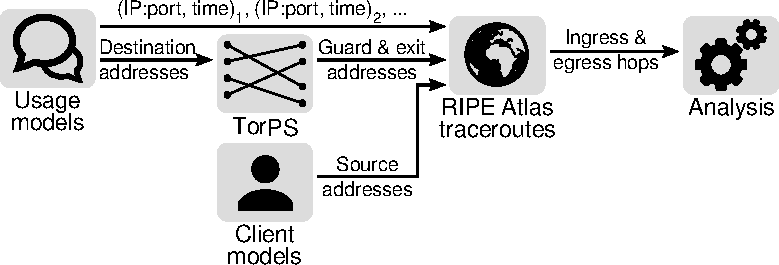
\includegraphics[width=\linewidth]{figures/simulations.pdf}
	\caption{The relation among our simulation components.  Our goal is to
	determine the ASes a Tor user's traffic traverses into and out of the Tor
	network.  Duplicate ASes on both sides can deanonymize streams.}
	\label{fig:simulations}
\end{figure}


We assume that an AS that can see both traffic entering the Tor network 
and DNS traffic exiting the Tor network for the purposes of mounting
a \name attack. 
A Tor exit can perform DNS resolution in two ways: (1)~running a name server
locally; or relying on a third-party name server, such as its ISP's name
server or a public DNS name server such as Google's open public DNS
resolver ({\tt 8.8.8.8}).  In the case of Tor
exits that perform local DNS resolution a good position for an attacker
might be both (1)~anywhere on the AS path between a Tor client and a Tor
guard; and (2)~anywhere on the path between a Tor exit and any of the
name servers the exit has to communicate with to resolve the name.
These name servers include the root name server, the TLD servers, and
the second-level servers.  The ASes along the path from the exit relay
to the name servers will be able to see the domain names that the exit
relay is querying.
For Tor exits that rely on a third-party for DNS resolution, an
adversary might be on the path between a Tor client and a
Tor guard and on the path between a Tor exit and the third-party name
server.  (For now we assume that an adversary that is on the path between 
the third-party and the additional name servers it will correspond with 
will not be able to see the IP address of the exit relay and will only see 
the IP address of the third-party as the originator of the request.
%)\fixme{QUESTION: ``In addition, the DNS queries will look like they are coming
%from the IP address of the name server and not the IP address of the
%exit relay.''--This new wording seems unclear to me now--wanted to say 
%that ASes on the path from the 3rd-party to the DNS servers will see that 
%the queries are coming from the 3rd-party and not the exit IP, which is 
%why we ignore them . . .}

\subsubsection{Simulating Tor user activity with TorPS}

To measure the likelihood that an AS can be in a position to perform a
\name attack, we use TorPS, the Tor Path Simulator, which mimics how the
Tor client software constructs circuits~\cite{TorPS}.  TorPS provides realistic
combinations of guards and exits based on the state of the Tor network
at a given time. TorPS is based on Tor stable release version 0.2.4.23. 
For each sample, 
it uses one guard; this guard selection expires after 270 days. We use TorPS to emulate
the behavior of a Tor client for the month of March 2016.  As in
previous work, \fixme{Wording, please: ``we perform 100,000 samples in the TorPS Monte Carlo 
simulation'' or ``we perform 100,000 Monte Carlo simulations in order to 
analyze this.''}
%potential Tor users and how the Tor client would have behaved.
%we perform 100,000 samples in the TorPS Monte Carlo
%simulation.  

To select the location of the clients in the experiment, we placed
clients in major ISPs in the top-five most popular countries for Tor
usage. For the United States, we chose Comcast (AS~7922); for Russia,
Rostelecom (AS~42610); for Germany, Deutsche Telekom (AS~3320); for
France, Orange (AS~3215); and for Great Britain, British Telecom (AS~2856).

Each client visited several websites every day in March 2016.  We
modeled our client behavior off of the ``Typical'' model used
in~\cite{Johnson2013a}.  At 9 a.m. EST the client visits
{\tt mail.google.com} and {\tt www.twitter.com}.  At 12 p.m. EST, the client visits
{\tt calendar.google.com} and {\tt docs.google.com} 
At 3 p.m. EST, the client visits {\tt www.facebook.com} and {\tt www.instagram.com}. 
Finally, at 6 p.m. EST the client 
visits {\tt www.google.com}, {\tt www.startpage.com}, and {\tt www.ixquick.com}, 
and at 6:20 p.m. EST the client visits {\tt www.google.com}, {\tt www.startpage.com}, 
and {\tt www.ixquick.com} again. Each client 
sample thus had 372 opportunities to be compromised (31 days, and 12
sites per day).  TorPS 
provided a new circuit every ten minutes, regardless of how many distinct
connections the client made to different sites; it did not provide a new
circuit for different websites if the client visited the group of sites
within the same ten-minute window.  This behavior differs from the
latest Tor Browser, which provides new circuit for each distinct
website, even within the same ten-minute time interval.  Thus, our
results will be conservative in this respect.

We assume that one DNS request occurs every time the client visits a site. For example, 
in our model, at 9 a.m. one DNS request will occur for {\tt mail.google.com} and 
one DNS request will occur for {\tt www.twitter.com}. At 6 p.m. three DNS requests 
will occur, and at 6:20 p.m. those same three DNS requests will occur again. Please note 
that for now we do not take embedded requests nor caching into account.
%\xxx{Shouldn't each
%  website actually result in hundreds of DNS lookups? This process could
%be more clear.} 

\subsubsection{Inferring AS-level paths: traceroute + {\tt pyasn}}


% - 197 out of all 377 (52%) Tor exit ASes have Atlas probes.
% - 220 out of all 434 (51%) Tor guard ASes have Atlas probes.

% - Atlas ASes cover 57.53% of Tor exit bandwidth.
% - Atlas ASes cover 73.59% of Tor guard bandwidth.

\begin{table}[t]
	\renewcommand{\tabcaptext}{The coverage of RIPE Atlas nodes that are colocated with Tor guard and exit
	relays.}
      \topcap{\tabcaptext}
	\centering
	\begin{tabular}{l|r r}
	\toprule
	\textbf{Atlas probe coverage} & \textbf{Tor guard ASes} & \textbf{Tor exit ASes} \\
	\midrule
	By bandwidth & 73.59\% & 57.53\% \\
	By number & 50.69\% & 52.25\% \\
	\bottomrule
	\end{tabular}
        \bottomcap{\tabcaptext}
	\label{tab:atlas-coverage}
\end{table}

This experiment also requires inferring the AS-level paths from
each exit relay to each destination. We decided against the (more
commonly applied) AS path inference because Juen \ea showed that it can
be quite inaccurate~\cite{Juen2015a}.  Using traceroute can yield more
accurate paths.  Measuring traceroutes from client to guard notes is
straightforward: we select a probe in a client AS and perform
traceroutes to each respective guard. 

Measuring traceroutes from exit relay to destination is far more
difficult because Tor does not implement a mechanism to facilitate
traceroute~\cite{Murdoch2007a}.  One approach, used in previous
work~\cite{Juen2015a}, is to ask relay operators to perform traceroutes.
Unfortunately, this approach only yielded traceroutes from relays
representing 26\% of exit bandwidth.  

Instead, we observe that RIPE
Atlas~\cite{atlas} has probes in many ASes that have Tor exit relays.
We used this insight to design a measurement experiment to run
traceroutes from RIPE Atlas probes that were located in the same ASes as
Tor exits, to each of the destinations in question.  As shown in
Table~\ref{tab:atlas-coverage}, for a day in May 2016, we found that
RIPE Atlas had probes in 52\% of ASes that contain Tor exit relays.  We
found that RIPE Atlas has probes in 51\% of ASes that contain Tor guard
relays.  More importantly, we found that Atlas ASes cover 58\% of Tor
exit \textit{bandwidth} and 74\% of Tor guard bandwidth. (This statistic
is important because Tor relay usage is not evenly split among all of
the relays.) We considered using PlanetLab to initiate traceroutes, but
unfortunately most PlanetLab nodes are located in research and education
networks~\cite{banerjee2004interdomain} and are thus not well-suited for
performing these types of measurements.
  

We performed traceroutes from the five client ASes above to all guard IP
      addresses from the Tor consensus files. To measure the paths from
      exit relays to DNS resolvers that DNS queries would traverse, we
      performed the following traceroutes, emulating a number of
      different DNS configurations:
\begin{itemize}
    \item \emph{ISP DNS:} To measure the path from an exit relay to its
      ISP's DNS resolver, we perform traceroutes from a RIPE Atlas node
      in the ISP of the exit relay to the ISP's corresponding DNS resolver.

    \item \emph{Google DNS:} To measure the path from an exit relay to
      Google public DNS, we perform traceroutes from a RIPE Atlas node
      in the ISP of the exit relay to Google's public DNS resolver (\ie,
      {\tt 8.8.8.8}).

    \item \emph{Local DNS:} To measure the paths that would result if an
      exit relay were running its own local resolver (\eg, {\tt
        unbound}, {\tt bind}), we used {\tt dig +trace} to emulate the
      iterative DNS lookup that would take place. We tracked all IP
      addresses from referrals at each level of the hierarchy and
      performed traceroutes to those IP addresses.

    \item \emph{Status quo:} This experiment represents a combination of
      the above configurations, which represents our estimate of how the
      Tor networks' exit relays are currently configured. We used {\tt
        exitmap}, a website that we control, and our own authoritative
      name server to determine the IP addresses of the name servers that
      the Tor exit relays are using.
\end{itemize}
\noindent
We then mapped each IP address in every traceroute to a corresponding
AS.  The Python {\tt pyasn} module relies on BGP routing tables to
perform these mappings; by using a routing table that coincides with the
time when we performed our traceroutes, we can obtain accurate AS-level
mappings.  This method is subject to inaccuracies due to BGP route
hijacks or leaks, but we expect those events to be relatively unlikely
for the time period and IP prefixes that we are concerned with.

\subsection{Results}

\begin{figure}[t]
\centering
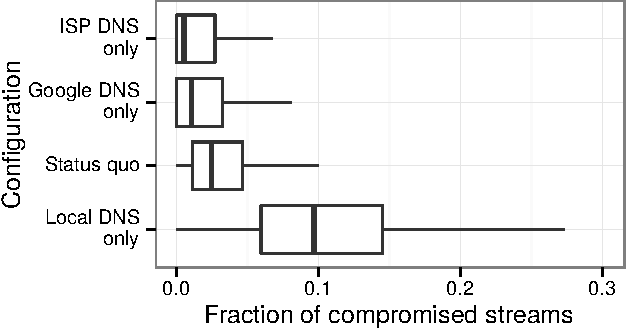
\includegraphics[width=0.75\linewidth]{figures/differences-comp-streams.pdf}
\caption{The fraction of compromised streams for the status quo and three
hypothetical DNS configurations for all exit relays.  We removed outliers, so
the box plot only shows the distributions' quartiles.  The safest configuration
is ``ISP DNS only,'' \ie have all exit relays use their ISP's DNS resolver.  The
median of compromised streams for this configuration is 0.005.}
\label{fig:compromised-streams}
\end{figure}

\begin{figure}[t]
\centering
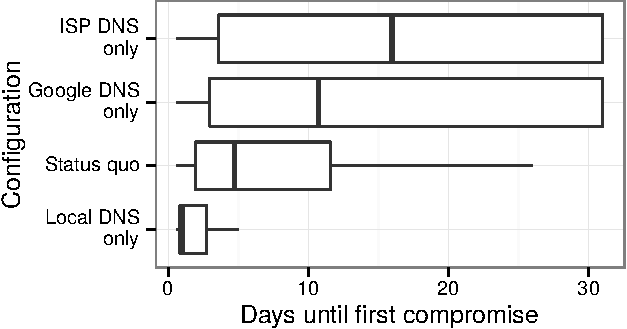
\includegraphics[width=0.75\linewidth]{figures/differences-time-comp.pdf}
\caption{The time until first stream compromise for the status quo and three
hypothetical DNS configurations for all exit relays.  We removed outliers, so
the box plot only shows the distributions' quartiles.  Again, the safest
configuration is ``ISP DNS only;'' the median of the distribution is
close to 16 days.}
\label{fig:time-until-compromise}
\end{figure}

Figures~\ref{fig:compromised-streams}
and~\ref{fig:time-until-compromise} show that
\fixme{new figures coming}
ISPs fared much better than the other situations. Google was next. There is a potential 
tradeoff between the safety of using a well-managed DNS resolver such as Google's vs. 
a potentially not as well-managed DNS resolver from the ISP.  

We believe that the Status Quo results are significantly better than the 
Local results because only around 12\% of Tor exit relays actually do their own resolution.
The differing results for the different client ASes shows that client AS needs to be 
taken into account. 

